% -----------------------------------------------------------------------------
\section{Data Model Examples}
\label{sec:examples}
% -----------------------------------------------------------------------------

%\subsection{LacI/TetR Toggle Switch}

This section illustrates how to use the SBOL data model by specifying the design of a LacI/TetR toggle switch similar to those constructed in \cite{Gardner2000}. This design is visualized in \ref{images:toggleswitch_modular}. 

\Ctodo{Add a standard toggle switch diagram of two things repressing each other and a simple explanation for people who do not already know the toggle switch.}

\begin{figure}[ht]
\begin{center}
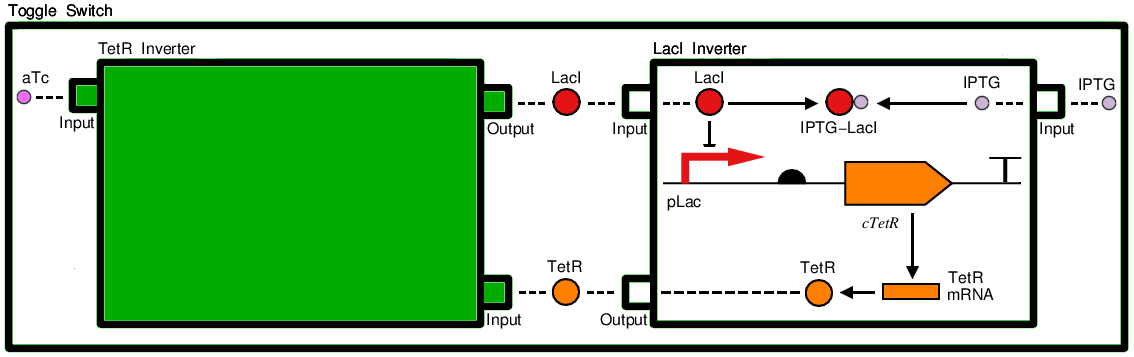
\includegraphics[scale=0.4]{images/toggleswitch_modular}
\caption[]{Design of a LacI/TetR toggle switch. This design is composed of two inverter sub-designs, each containing a single gene. These genes mutually repress each other's expression via their encoded protein transcription factors, LacI and TetR. Furthermore, both LacI and TetR are bound by specific small molecules that sequester them and prevent them from acting as repressors. In this design, arrows represent different molecular interactions, including the repression of pLac via LacI, the non-covalent binding of IPTG to LacI, the transcription of TetR mRNA, and the translation of TetR. Dashed lines serve to map between transcription factors in the inverter sub-designs and those in the overall toggle switch design.}
\label{images:toggleswitch_modular}
\end{center}
\end{figure}

The LacI/TetR toggle switch is modeled in SBOL as two parallel hierarchies of structure and function. The structural hierarchy of the toggle switch is represented using \sbol{ComponentDefinition}s:
\begin{itemize}
\item The base elements of the hierarchy are DNA components, transcription factors, and small molecules. As an example, \ref{uml:ex_comp_defs} is a UML diagram of the \sbol{ComponentDefinition}s that represent these elements.
\item Base elements are composed to form more complex structures at the top of the hierarchy, including genes and molecular complexes between transcription factors and small molecules. As an example, \ref{uml:ex_comp_def_compo} is a UML diagram of the composite \sbol{ComponentDefinition}s that represent the TetR gene and IPTG-LacI complex.
\end{itemize}

\begin{figure}[ht]
\begin{center}
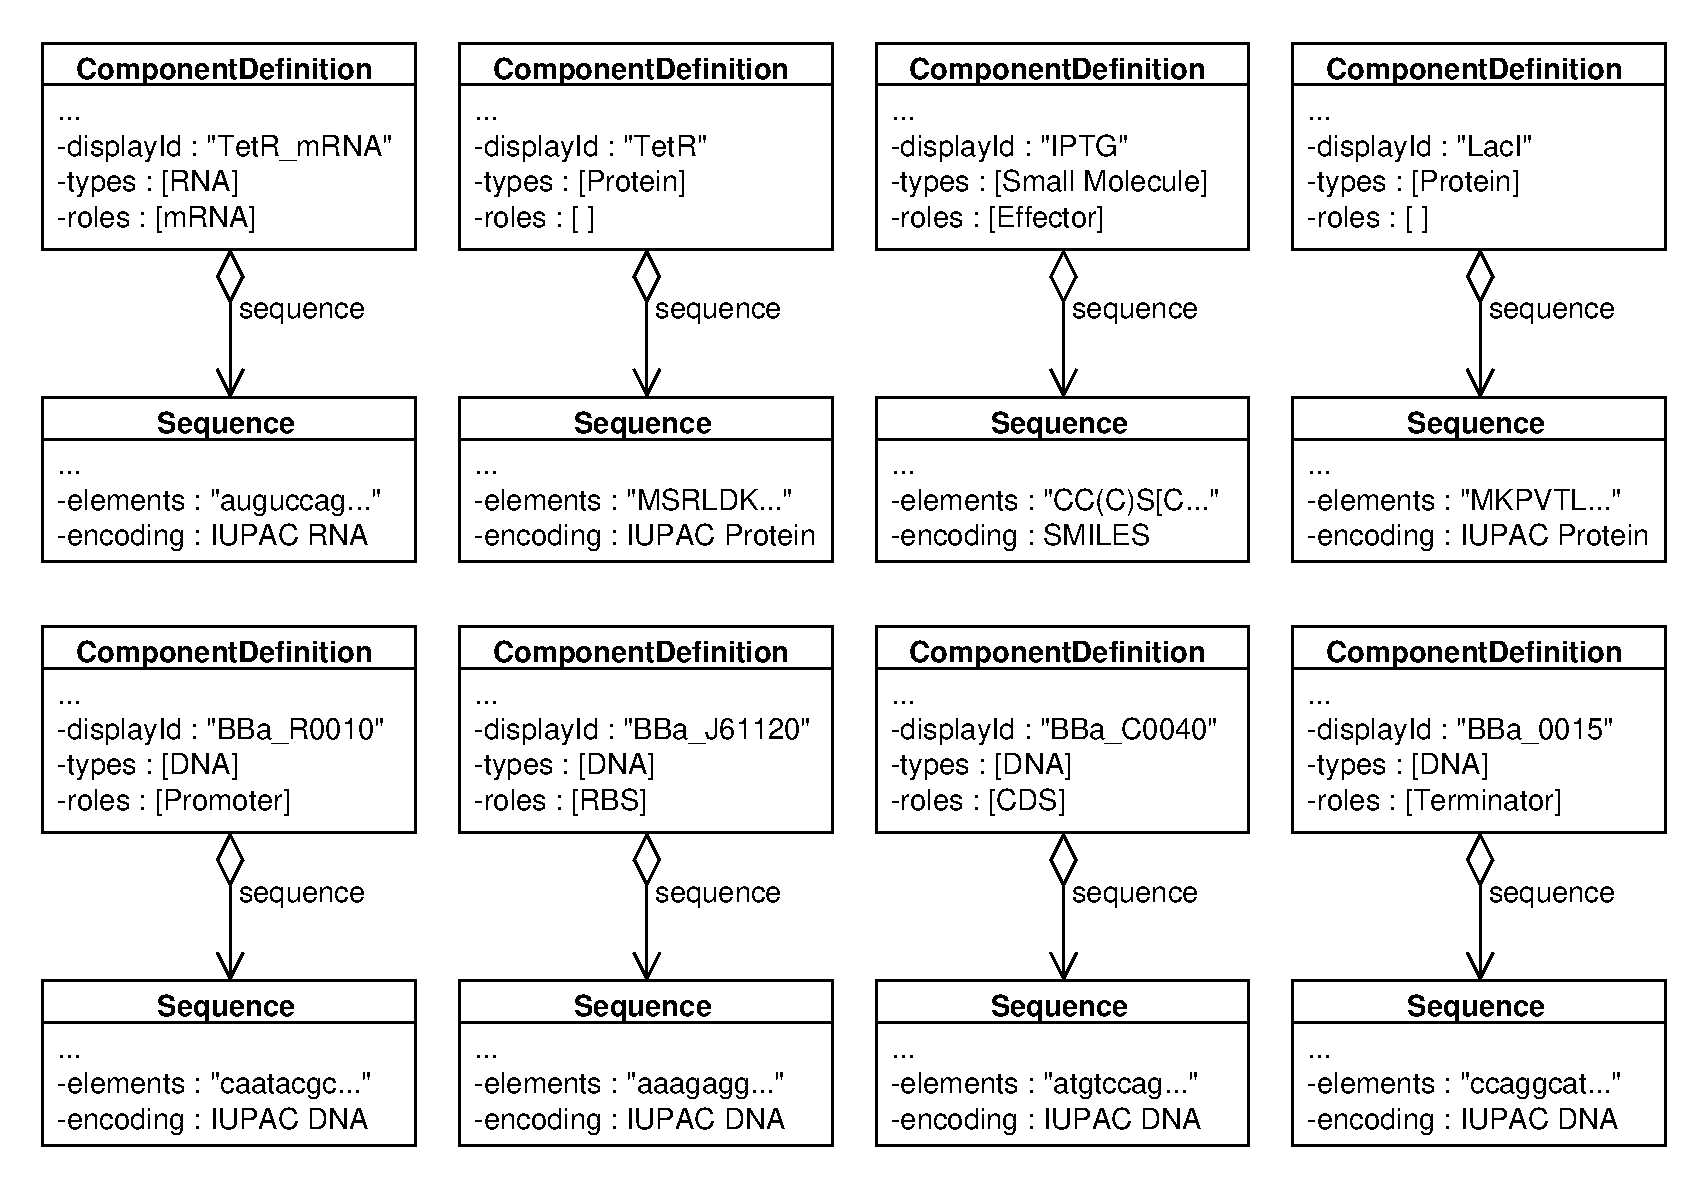
\includegraphics[width=\textwidth]{example_uml/toggle_1}
\caption[]{\sbol{ComponentDefinition}s for the LacI inverter. These include \sbol{ComponentDefinition}s based on DNA parts from the iGEM Registry and  \sbol{ComponentDefinition}s that represent TetR mRNA, TetR, LacI, and and IPTG. Each \sbol{ComponentDefinition} is associated with a \sbol{Sequence} that has an IUPAC nucleic acid or amino acid encoding, except the \sbol{ComponentDefinition} for IPTG, which is associated with a \sbol{Sequence} that has a SMILES encoding.}
\label{uml:ex_comp_defs}
\end{center}
\end{figure}

\begin{figure}[ht]
\begin{center}
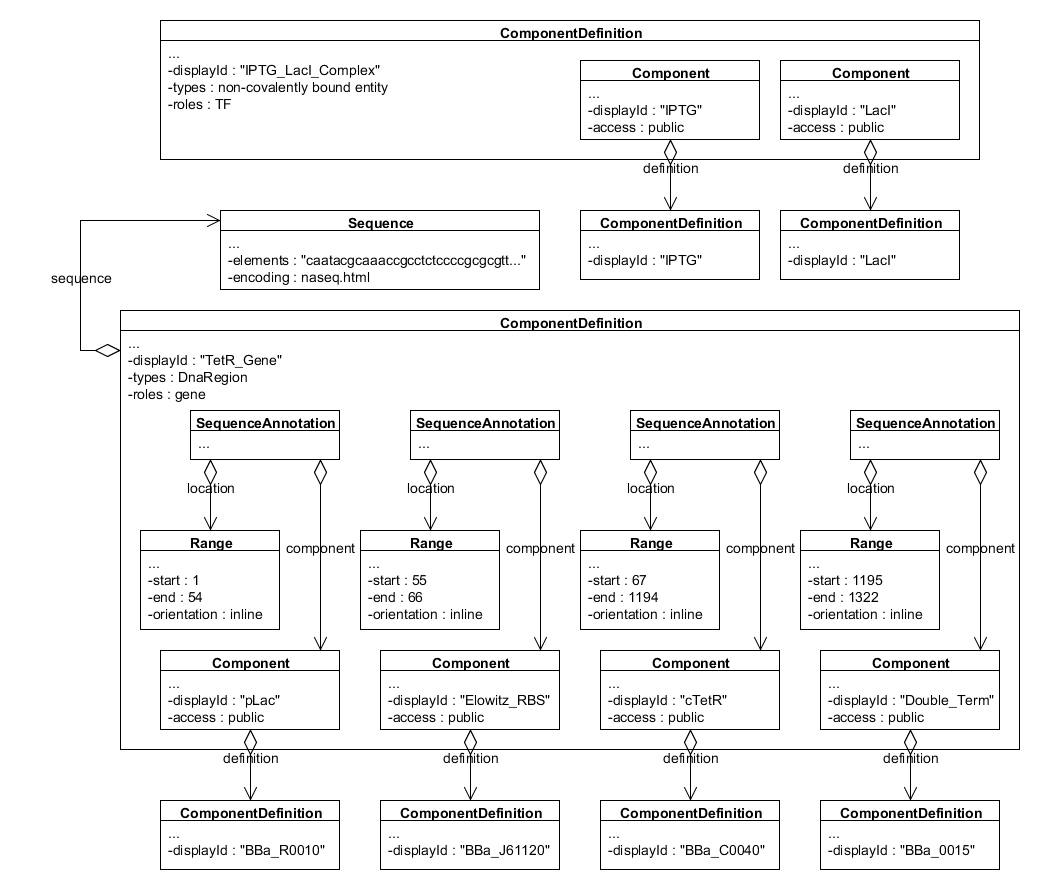
\includegraphics[width=\textwidth]{example_uml/toggle_2}
\caption[]{Composite \sbol{ComponentDefinition}s for the LacI inverter. In the case of the \sbol{ComponentDefinition} that represents the TetR gene, its sub-\sbol{Component}s are located as \sbol{Range}s along its \sbol{Sequence} using \sbol{SequenceAnnotation}s. The \sbol{ComponentDefinition} that represents the IPTG-LacI complex, however, has no \sbol{Sequence} and its sub-\sbol{Component}s are aggregated without any data about their relative positions.}
\label{uml:ex_comp_def_compo}
\end{center}
\end{figure}

The functional hierarchy of the toggle switch is represented using
\sbol{ModuleDefinition}s:
\begin{itemize}
\item The base elements of the hierarchy are LacI-dependent repression of TetR expression (the LacI inverter) and TetR-dependent repression of LacI (the TetR inverter). As an example, \ref{uml:ex_mod_def} is a UML diagram of the \sbol{ModuleDefinition} that represents the LacI inverter.
\item Base elements are composed to form the toggle switch at the top of the hierarchy.  As an example, \ref{uml:ex_mod_def_compo} is a UML diagram of the \sbol{ModuleDefinition} that represents the toggle switch.
\end{itemize}

\begin{figure}[ht]
\begin{center}
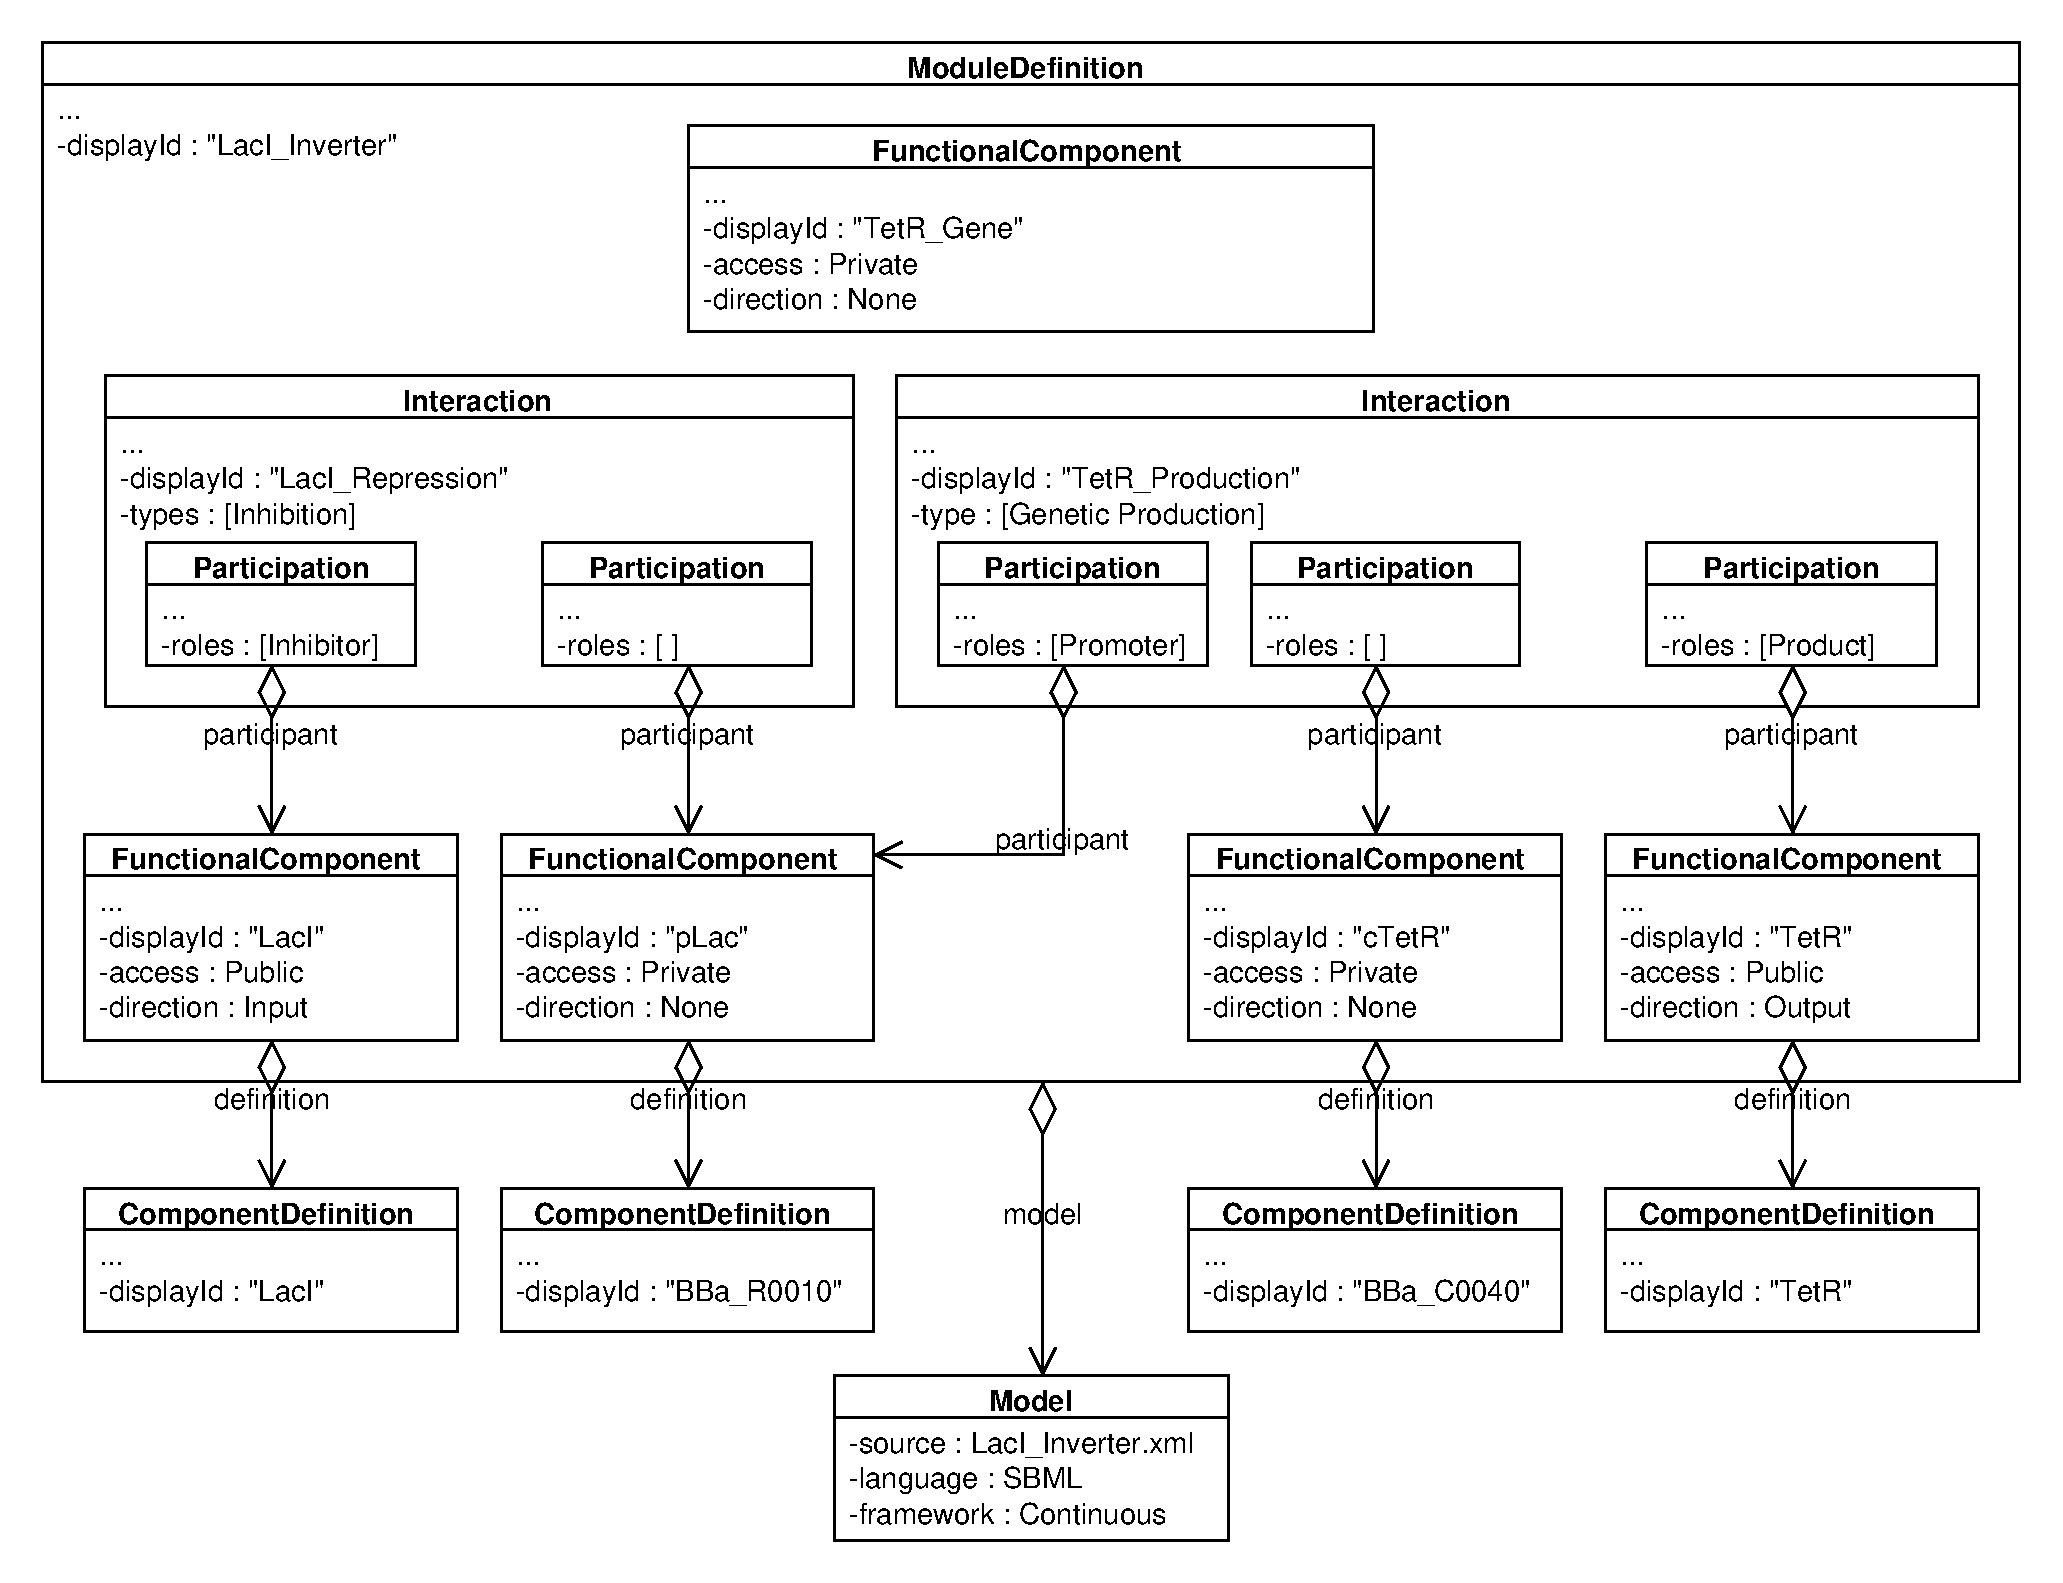
\includegraphics[width=\textwidth]{example_uml/toggle_3}
\caption[]{\sbol{ModuleDefinition} for the LacI inverter. This \sbol{ModuleDefinition} instantiates the \sbol{ComponentDefinition}s for the LacI/TetR transcription factors and the sub-\sbol{ComponentDefinition}s of the TetR gene as \sbol{FunctionalComponent}s that participate in a repression \sbol{Interaction} and a genetic production \sbol{Interaction}. In this case, the transcription and translation of TetR are represented as a single genetic production \sbol{Interaction} that abstracts away the presence of the intermediate TetR mRNA. In addition, the \sbol{ComponentDefinition} for the TetR gene is instantiated by the LacI inverter \sbol{ModuleDefinition} to indicate that the latter describes the function of the TetR gene as a whole. Finally, this \sbol{ModuleDefinition} is also associated with a continuous \sbol{Model} written in the SBML source file ``LacI\_Inverter.xml.''}
\label{uml:ex_mod_def}
\end{center}
\end{figure}

\begin{figure}[ht]
\begin{center}
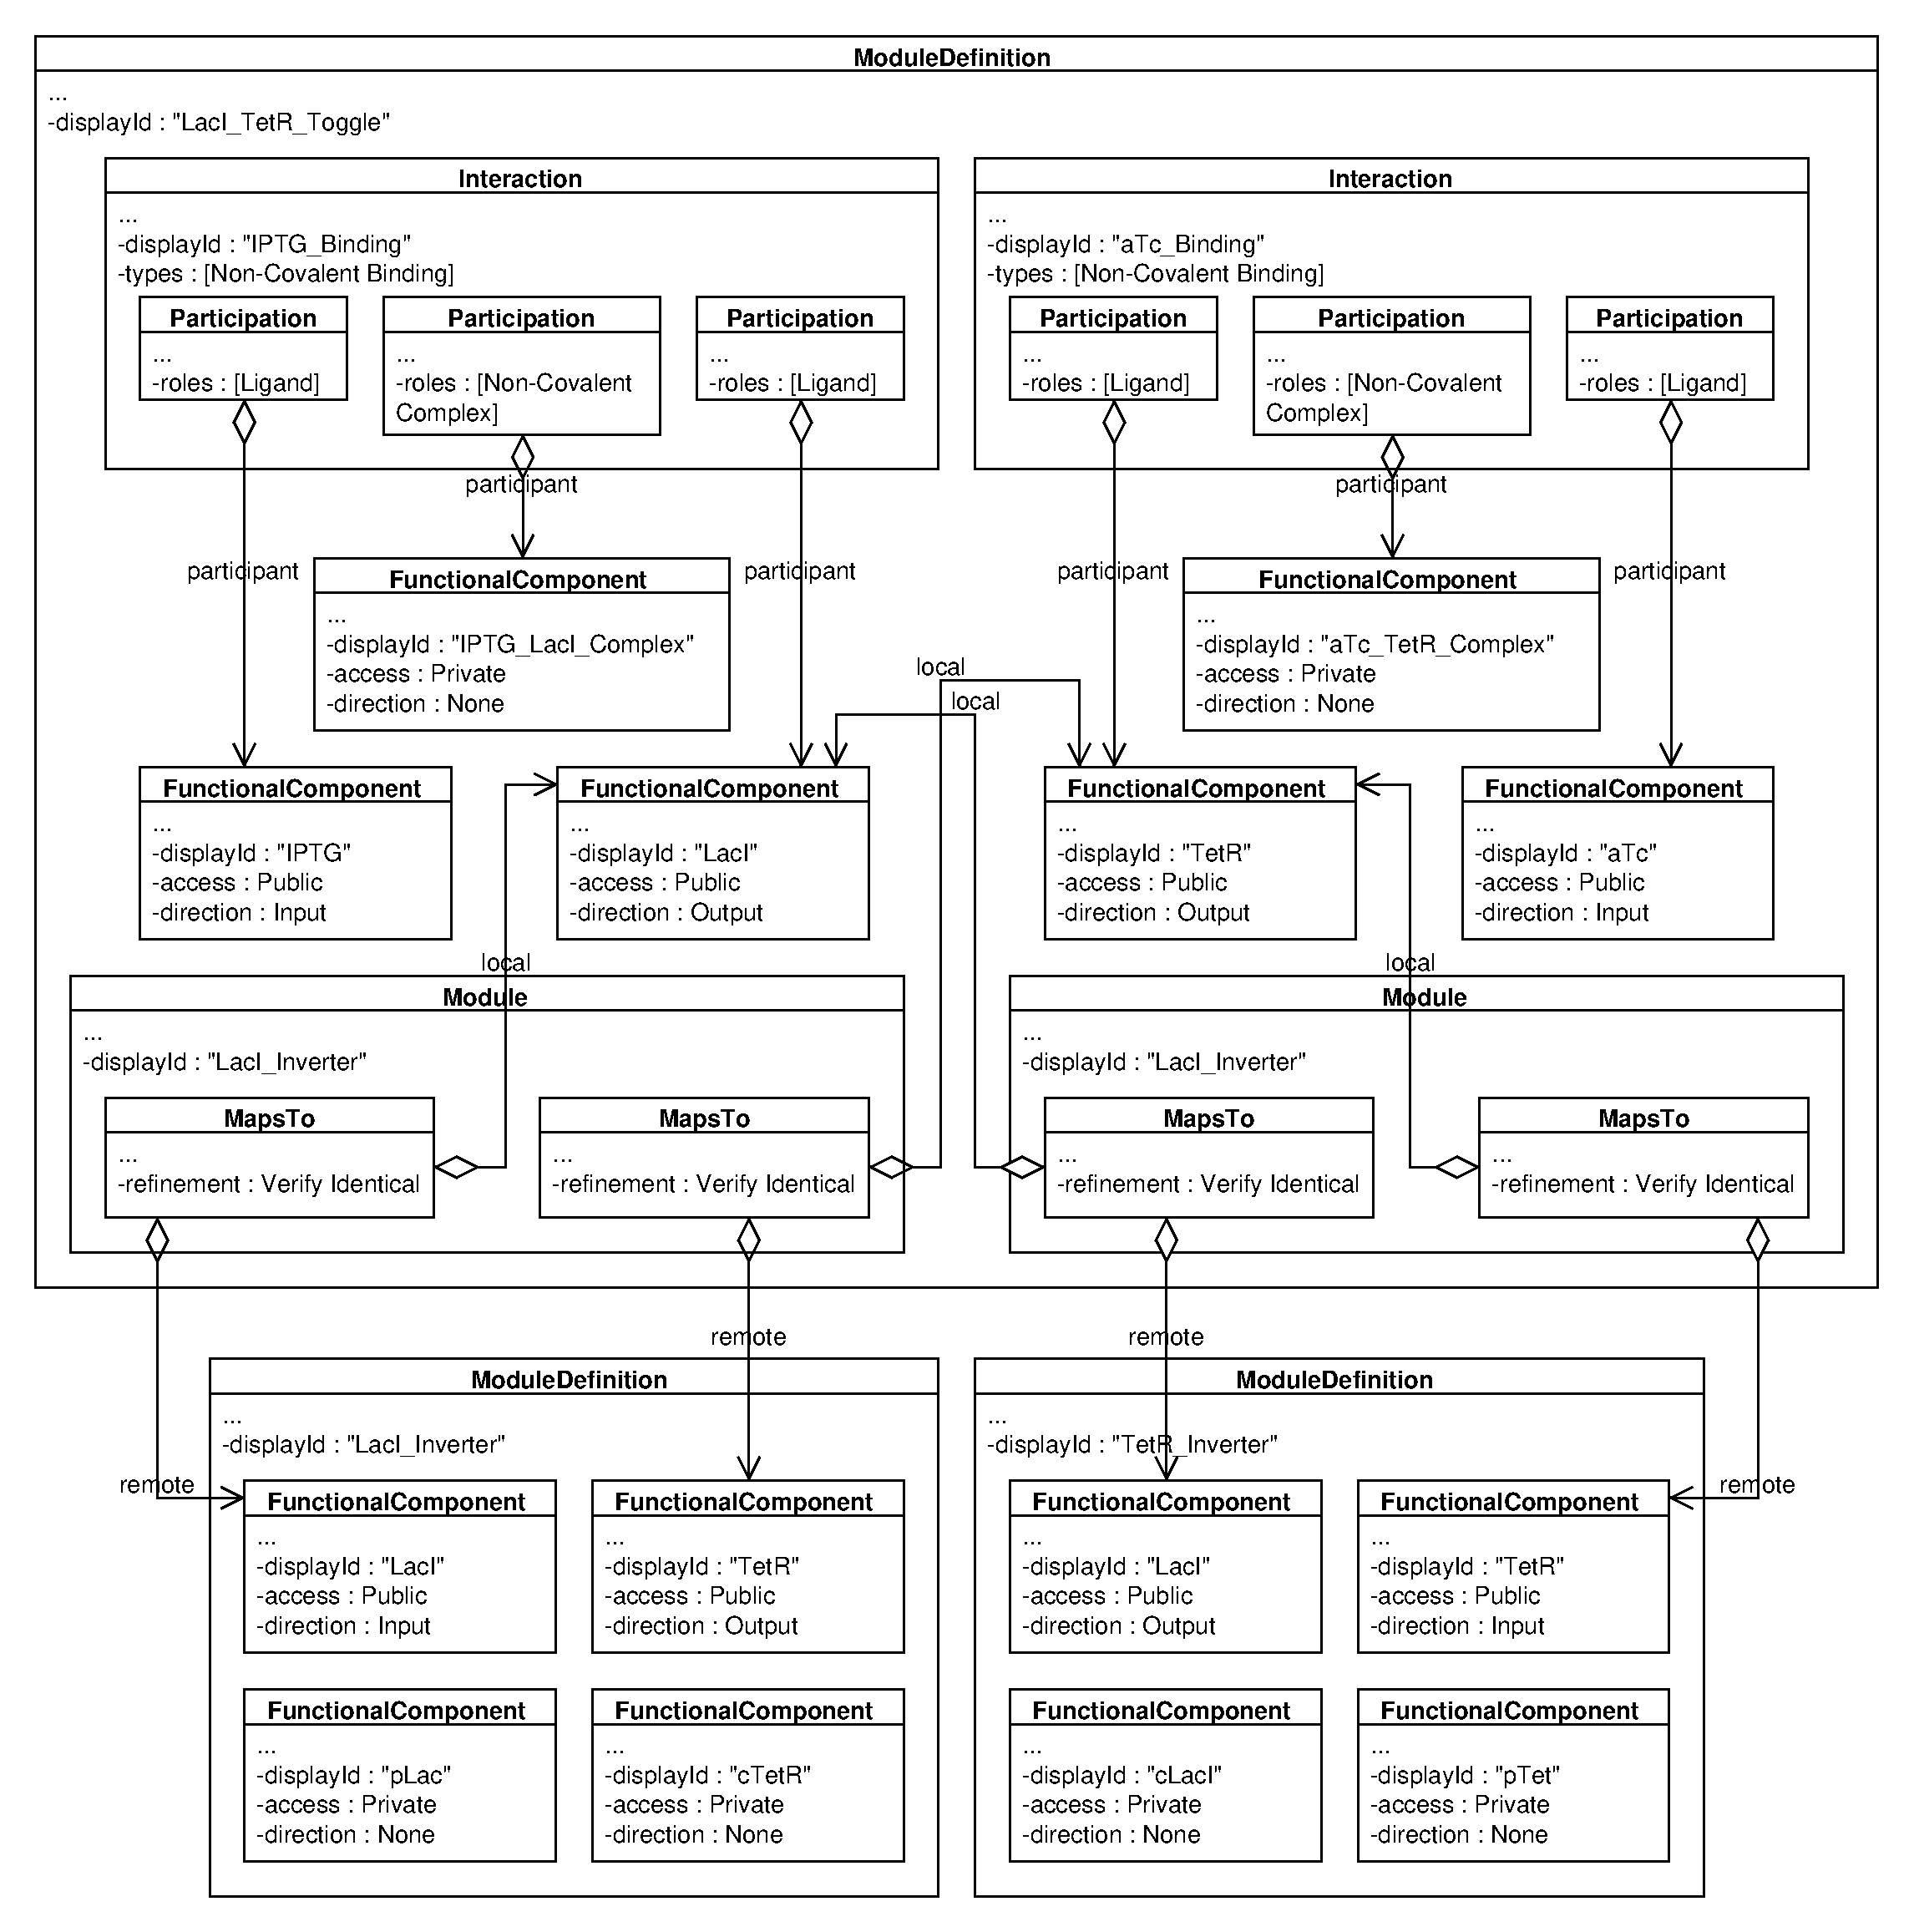
\includegraphics[width=\textwidth]{example_uml/toggle_4}
\caption[]{Composite \sbol{ModuleDefinition} for the LacI/TetR toggle switch. This \sbol{ModuleDefinition} instantiates the LacI and TetR inverter \sbol{ModuleDefinition}s as sub-\sbol{Module}s. It also instantiates the \sbol{ComponentDefinition}s for the LacI/TetR transcription factors and IPTG/aTc small molecules as \sbol{FunctionalComponent}s that participate in non-covalent binding \sbol{Interaction}s. To complete the composition of the \sbol{ModuleDefinition} for the toggle switch, \sbol{MapsTo} objects are used to indicate that the output of the LacI inverter is identical to the input of the TetR inverter and vice versa.
}
\label{uml:ex_mod_def_compo}
\end{center}
\end{figure}

% Each \sbol{ModuleDefinition} also contains the \sbol{FunctionalComponent}s that participate in \sbol{Interaction}s and are defined by the same \sbol{ComponentDefinition}s as the parallel \sbol{Component}s in the structural hierarchy of the toggle switch. Finally, \sbol{MapsTo} entities are used to refine which \sbol{FunctionalComponent}s of the functional hierarchy are identical or map them to \sbol{Component}s in the structural hierarchy.

\Ctodo{ComponentDefinition.types in the following figure are not consistent with the list of BioPax ontological terms described previously in the Data Model section.  Nick will fix this.}

%  The first use case is to indicate with greater fidelity how a module describes the function of a composite component, namely by asserting that particular component instantiations within the module correspond to particular component instantiations within the component. 

% As an example of this use case, one might compose the structure and function of the LacI-repressible gene of the genetic toggle switch. In this example, the LacI-repressible gene and two of its subcomponents, the pLac promoter and cTetR CDS, are to be composed with the LacI inverter module. In order to compose these components with the LacI inverter module and indicate that it describes their behavior, they are instantiated inside the module. In addition, port maps are placed on the instantiation of the LacI-repressible gene to connect between its pLac plus cTetR subcomponent instantiations and the corresponding component instantiations in the module. Doing so makes it clear which subcomponent instantiations in the gene are being described by which component instantiations in the module. In this way, GDA tools for sequence editing and biochemical modeling can guarantee that their users are handling corresponding elements of a given genetic design, while GDA tools for genetic technology mapping can make explicit connections between the structural and functional elements of a design.